%%% The main file. It contains definitions of basic parameters and includes all other parts.

%% Settings for single-side (simplex) printing
% Margins: left 40mm, right 25mm, top and bottom 25mm
% (but beware, LaTeX adds 1in implicitly)
\documentclass[12pt,a4paper]{report}
\setlength\textwidth{145mm}
\setlength\textheight{247mm}
\setlength\oddsidemargin{15mm}
\setlength\evensidemargin{15mm}
\setlength\topmargin{0mm}
\setlength\headsep{0mm}
\setlength\headheight{0mm}
% \openright makes the following text appear on a right-hand page
\let\openright=\clearpage

%% Settings for two-sided (duplex) printing
% \documentclass[12pt,a4paper,twoside,openright]{report}
% \setlength\textwidth{145mm}
% \setlength\textheight{247mm}
% \setlength\oddsidemargin{14.2mm}
% \setlength\evensidemargin{0mm}
% \setlength\topmargin{0mm}
% \setlength\headsep{0mm}
% \setlength\headheight{0mm}
% \let\openright=\cleardoublepage

%% Character encoding: usually latin2, cp1250 or utf8:
\usepackage[utf8]{inputenc}

%% Further useful packages (included in most LaTeX distributions)
\usepackage{amsmath}        % extensions for typesetting of math
\usepackage{amsfonts}       % math fonts
\usepackage{amsthm}         % theorems, definitions, etc.
\usepackage{bbding}         % various symbols (squares, asterisks, scissors, ...)
\usepackage{bm}             % boldface symbols (\bm)
\usepackage{graphicx}       % embedding of pictures
\usepackage{fancyvrb}       % improved verbatim environment
\usepackage{natbib}         % citation style AUTHOR (YEAR), or AUTHOR [NUMBER]
\usepackage[nottoc]{tocbibind} % makes sure that bibliography and the lists
			    % of figures/tables are included in the table
			    % of contents
\usepackage{dcolumn}        % improved alignment of table columns
\usepackage{booktabs}       % improved horizontal lines in tables
\usepackage{paralist}       % improved enumerate and itemize
\usepackage[usenames]{xcolor}  % typesetting in color
\usepackage{url}
\usepackage{enumerate}
\usepackage[shortlabels]{enumitem}
\usepackage{booktabs, caption, fixltx2e}
\usepackage[flushleft]{threeparttable}
\usepackage[scaled=.95]{inconsolata}
\usepackage{listings}
\usepackage{tikz, tikz-qtree}
\usepackage{float}
\usepackage{svg}

\newcommand*{\incon}[1]{{\fontfamily{fi4}\selectfont #1}}

\lstset{language=[5.2]Lua, basicstyle=\ttfamily}

% Listing float:
\newfloat{listing}{tbhp}{lst}
\floatname{listing}{Listing}

%%% Basic information on the thesis

% Thesis title in English (exactly as in the formal assignment)
\def\ThesisTitle{The Dungeon Throne: A 3D Dungeon Management Game}

% Author of the thesis
\def\ThesisAuthor{Jaroslav Jindrák}

% Year when the thesis is submitted
\def\YearSubmitted{2016}

% Name of the department or institute, where the work was officially assigned
% (according to the Organizational Structure of MFF UK in English,
% or a full name of a department outside MFF)
\def\Department{Department of Distributed and Dependable Systems}

% Is it a department (katedra), or an institute (ústav)?
\def\DeptType{Department}

% Thesis supervisor: name, surname and titles
\def\Supervisor{Mgr. Pavel Ježek, Ph.D}

% Supervisor's department (again according to Organizational structure of MFF)
\def\SupervisorsDepartment{Department of Distributed and Dependable Systems}

% Study programme and specialization
\def\StudyProgramme{Computer~Science}
\def\StudyBranch{Programming and Software Systems}

% An optional dedication: you can thank whomever you wish (your supervisor,
% consultant, a person who lent the software, etc.)
\def\Dedication{%
Dedication.
TODO:
}

% Abstract (recommended length around 80-200 words; this is not a copy of your thesis assignment!)
\def\Abstract{%
Abstract.
TODO:
}

% 3 to 5 keywords (recommended), each enclosed in curly braces
\def\Keywords{%
    {dungeon management game} {Lua scripting} {Ogre} {CEGUI}
}

%% The hyperref package for clickable links in PDF and also for storing
%% metadata to PDF (including the table of contents).
\usepackage[pdftex,unicode]{hyperref}   % Must follow all other packages
\hypersetup{breaklinks=true}
\hypersetup{pdftitle={\ThesisTitle}}
\hypersetup{pdfauthor={\ThesisAuthor}}
\hypersetup{pdfkeywords=\Keywords}
\hypersetup{urlcolor=blue}

% Definitions of macros (see description inside)
%%% This file contains definitions of various useful macros and environments %%%
%%% Please add more macros here instead of cluttering other files with them. %%%

%%% Minor tweaks of style

% These macros employ a little dirty trick to convince LaTeX to typeset
% chapter headings sanely, without lots of empty space above them.
% Feel free to ignore.
\makeatletter
\def\@makechapterhead#1{
  {\parindent \z@ \raggedright \normalfont
   \Huge\bfseries \thechapter. #1
   \par\nobreak
   \vskip 20\p@
}}
\def\@makeschapterhead#1{
  {\parindent \z@ \raggedright \normalfont
   \Huge\bfseries #1
   \par\nobreak
   \vskip 20\p@
}}
\makeatother

% This macro defines a chapter, which is not numbered, but is included
% in the table of contents.
\def\chapwithtoc#1{
\chapter*{#1}
\addcontentsline{toc}{chapter}{#1}
}

% Draw black "slugs" whenever a line overflows, so that we can spot it easily.
\overfullrule=1mm

%%% Macros for definitions, theorems, claims, examples, ... (requires amsthm package)

\theoremstyle{plain}
\newtheorem{thm}{Theorem}
\newtheorem{lemma}[thm]{Lemma}
\newtheorem{claim}[thm]{Claim}

\theoremstyle{plain}
\newtheorem{defn}{Definition}

\theoremstyle{remark}
\newtheorem*{cor}{Corollary}
\newtheorem*{rem}{Remark}
\newtheorem*{example}{Example}

%%% An environment for proofs

%%% FIXME %%% \newenvironment{proof}{
%%% FIXME %%%   \par\medskip\noindent
%%% FIXME %%%   \textit{Proof}.
%%% FIXME %%% }{
%%% FIXME %%% \newline
%%% FIXME %%% \rightline{$\square$}  % or \SquareCastShadowBottomRight from bbding package
%%% FIXME %%% }

%%% An environment for typesetting of program code and input/output
%%% of programs. (Requires the fancyvrb package -- fancy verbatim.)

\DefineVerbatimEnvironment{code}{Verbatim}{fontsize=\small, frame=single}

%%% The field of all real and natural numbers
\newcommand{\R}{\mathbb{R}}
\newcommand{\N}{\mathbb{N}}

%%% Useful operators for statistics and probability
\DeclareMathOperator{\pr}{\textsf{P}}
\DeclareMathOperator{\E}{\textsf{E}\,}
\DeclareMathOperator{\var}{\textrm{var}}
\DeclareMathOperator{\sd}{\textrm{sd}}

%%% Transposition of a vector/matrix
\newcommand{\T}[1]{#1^\top}

%%% Various math goodies
\newcommand{\goto}{\rightarrow}
\newcommand{\gotop}{\stackrel{P}{\longrightarrow}}
\newcommand{\maon}[1]{o(n^{#1})}
\newcommand{\abs}[1]{\left|{#1}\right|}
\newcommand{\dint}{\int_0^\tau\!\!\int_0^\tau}
\newcommand{\isqr}[1]{\frac{1}{\sqrt{#1}}}

%%% Various table goodies
\newcommand{\pulrad}[1]{\raisebox{1.5ex}[0pt]{#1}}
\newcommand{\mc}[1]{\multicolumn{1}{c}{#1}}


% Title page and various mandatory informational pages
\begin{document}
%%% Title page of the thesis and other mandatory pages

%%% Title page of the thesis

\pagestyle{empty}
\hypersetup{pageanchor=false}
\begin{center}

\centerline{\mbox{
\includegraphics[width=166mm]{../img/logo-en.pdf}}}

\vspace{-8mm}
\vfill

{\bf\Large BACHELOR THESIS}

\vfill

{\LARGE\ThesisAuthor}

\vspace{15mm}

{\LARGE\bfseries\ThesisTitle}

\vfill

\Department

\vfill

\begin{tabular}{rl}

Supervisor of the bachelor thesis: & \Supervisor \\
\noalign{\vspace{2mm}}
Study programme: & \StudyProgramme \\
\noalign{\vspace{2mm}}
Study branch: & Programming and Software \\
    &Systems
\end{tabular}

\vfill

% Zde doplňte rok
Prague \YearSubmitted

\end{center}

\newpage

%%% Here should be a bound sheet included -- a signed copy of the "bachelor
%%% thesis assignment". This assignment is NOT a part of the electronic
%%% version of the thesis. DO NOT SCAN.

%%% A page with a solemn declaration to the bachelor thesis

\openright
\hypersetup{pageanchor=true}
\pagestyle{plain}
\pagenumbering{roman}
\vglue 0pt plus 1fill

\noindent
I declare that I carried out this bachelor thesis independently, and only with the cited
sources, literature and other professional sources.

\medskip\noindent
I understand that my work relates to the rights and obligations under the Act No.~121/2000 Sb.,
the Copyright Act, as amended, in particular the fact that the Charles
University in Prague has the right to conclude a license agreement on the use of this
work as a school work pursuant to Section 60 subsection 1 of the Copyright Act.

\vspace{10mm}

\hbox{\hbox to 0.5\hsize{%
In ........ date ............	% FIXME!
\hss}\hbox to 0.5\hsize{%
signature of the author
\hss}}

\vspace{20mm}
\newpage

%%% Mandatory information page of the thesis

\openright

\vbox to 0.5\vsize{
\setlength\parindent{0mm}
\setlength\parskip{5mm}

Title:
\ThesisTitle

Author:
\ThesisAuthor

\DeptType:
\Department

Supervisor:
\Supervisor, \SupervisorsDepartment

Abstract:
\Abstract

Keywords:
\Keywords

\vss}

\newpage

%%% Dedication

\openright

\noindent
\Dedication

\newpage

\openright
\pagestyle{plain}
\pagenumbering{arabic}
\setcounter{page}{1}


%%% A page with automatically generated table of contents of the bachelor thesis

\tableofcontents

%%% Each chapter is kept in a separate file
\chapter{The Game}

An~example citation: \cite{Andel07}
TEST

\section{Dungeon Managment Genre}

\section{Modifiability in Games}

\section{Similar Games}

\subsection{Dungeon Keeper}
TODO: Design influence.

\subsection{Garry's Mod}
TODO: Modifiability influence. (Mainly game mechanics.)

\subsection{Minecraft}
TODO: Modifiability influence. (Mainly items.)

\subsection{Dungeon Siege}
TODO: ECS influence.

\section{Thesis Goals}

\chapter{Problem Analysis}

In the introduction section of this thesis, we defined a list of design elements \textbf{(E1)}~--~\textbf{(E6)} that we are going to
implement in our game. We have also presented the notion of modifiability and examined some of
the numerous Minecraft mods to see which parts of a game can be modified. In this section, we are
going to look at the different tools, libraries and engine design possibilities that could potentially
be used to implement our game.

\section{Modding Tools}

To satisfy our goals \textbf{(G2)} and \textbf{(G3)}, which require us to provide modding tools to our players that will allow
them to create easilly installable mods, we now need to decide the form of these tools. They should allow the mod creators
to create and modify entities to the extent required by our goal \textbf{(G2.1)} and to alter the game progression as required
by our goal \textbf{(G2.2)}. Additionally, to satisfy our goal \textbf{(G3)}, the resulting mods should be easilly installable.

\subsubsection{Editor}

A game editor is a tool that is commonly used to modify a game. It can be either an external application
or it can be a part of the game. In most cases it's used to edit maps or scenarios for the game.
But since the maps in our game are created by the player -- by destroying walls and creating buildings -- we are more interested in a
different aspect of editors and that is changing entities in the game.

\begin{figure}[H]
    \centering
    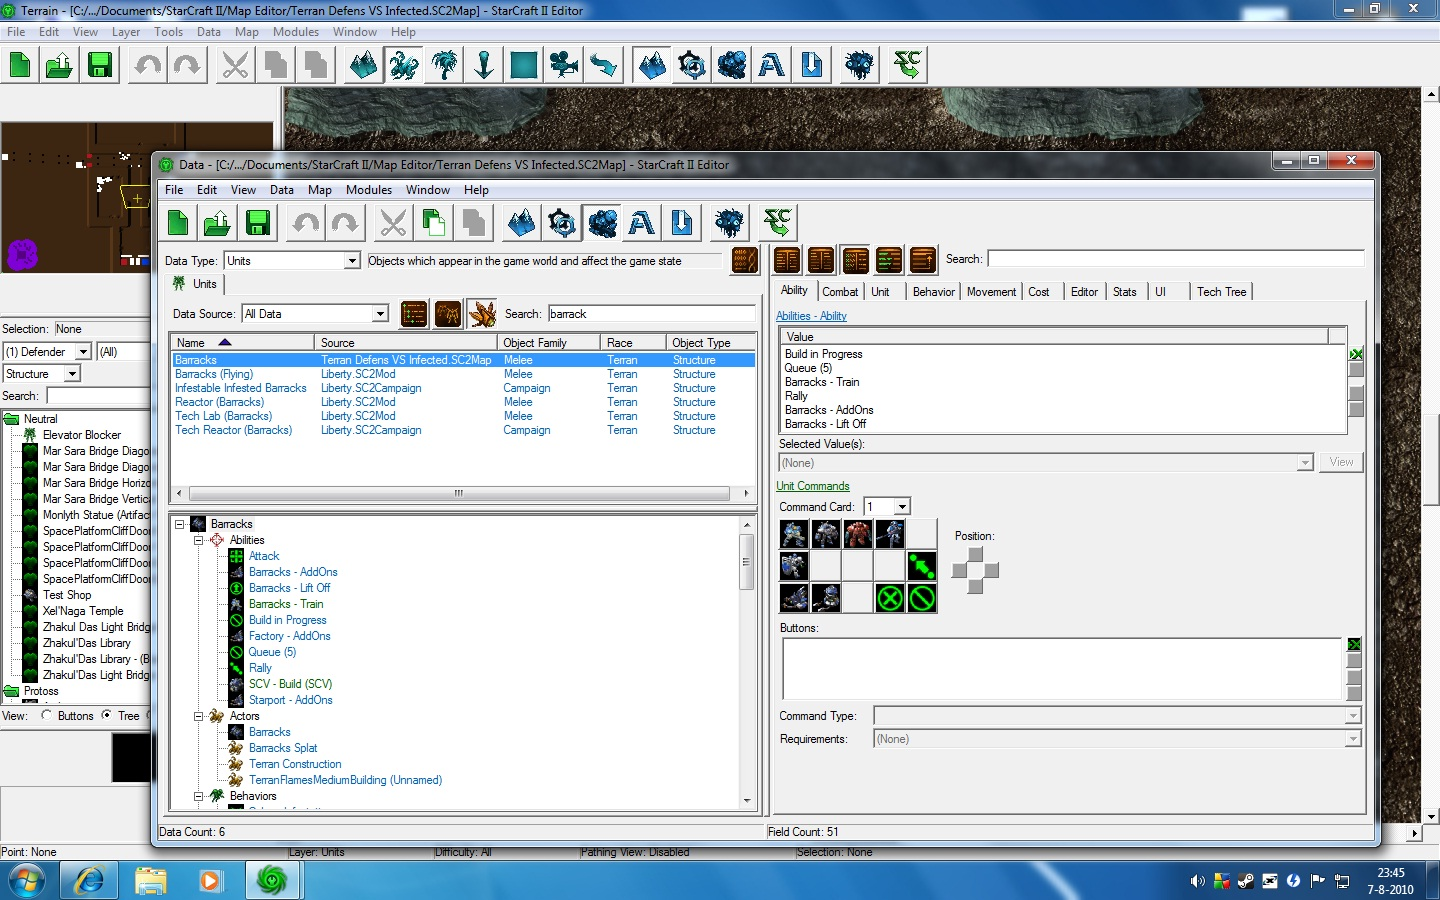
\includegraphics[width=0.9\textwidth]{../img/sc_editor.jpg}
    \caption{Besides map editing, some editors -- like the Starcraft editor in this figure -- can be used to edit entities.
             \\Source: \href{http://www.darvo.org/images/Tutorials\%20Starcraft\%202/Adding\%20Units\%20to\%20a\%20Building\%20part\%201.jpg}
             {http://www.darvo.org}}
    \label{sc-editor}
\end{figure}

In Figure~\ref{sc-editor} we can see an example of such editor.
It allows its user to select an entity and change its attributes, such as health, placing cost, type, model and the user can even 
select which predefined abilities and behavior the entity uses. An editor could easilly be used to define the composition of enemy
waves and the delays between waves, satisfying our goal \textbf{(G2.2)} and would allow easy mod installation -- as required by our goal
\textbf{(G3)} -- by producing files that can be placed in the game's directory.

While this approach could be easily implemented using configuration files for entities, our goal \textbf{(G2.1)} requires the ability
to alter the behavior of entities which includes creating entirely new behavior and thus only selecting predefined AI won't suffice.
To achieve this, we could require our users to write the behavior using a scripting language, which wouldn't be much different
from the option that will be examined after this one. Alternatively, we could create a graphical tool that would allow the user
construct the behavior out of blocks
representing decisions and actions which would then be translated to source code -- again, requiring a scripting language interfaced
to the engine. An example of such graphical tool is the blueprint system used by Unreal Engine~\cite{UE}.

\begin{figure}[H]
    \centering
    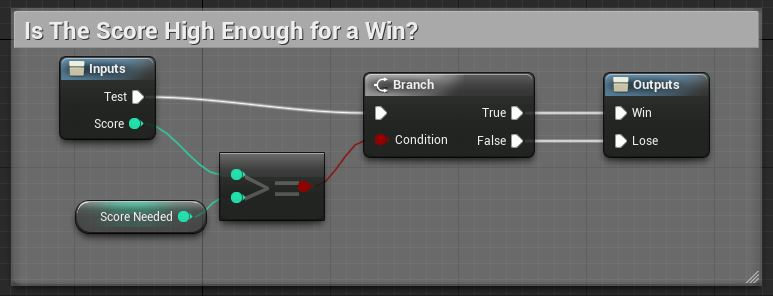
\includegraphics[width=10cm]{../img/blueprints.jpg}
    \caption{A simple blueprint checks if a person passes a test.
             \\Source: \href{http://docs.unrealengine.com/latest/images/Engine/Blueprints/UserGuide/Macros/score\_comparison\_example\_macro.jpg}
             {http://www.unrealengine.com}}
    \label{ue-blueprints}
\end{figure}

In Figure~\ref{ue-blueprints} we can see an example blueprint created in Unreal Engine, it comprises interconnected blocks that represent
conditions, loops, actions and other constructs that can be found in a typical programming language. The user uses these blocks to
create programs in a more user friendly manner. Unreal Engine then uses these blueprints to generate \cpp code that is then used in the game.

\subsubsection{API}

Another option is to create an interface in which functionality of the engine is bound to functions that can be called
from a scripting language embedded within the engine. This would allow our players to write scripts that can be loaded at the
start of our game or during its runtime and can change anything provided by the interface.

An example of such API can be found in the game Starbound~\cite{Starbound}, which allows its
players to create modifications by using its Lua API to write scripts. An example of a simple Starbound script,
which defines a new object in the game that spawns a chicken when the player interacts with it,
can be seen in Listing~\ref{sb-lua-mod-ex}. Here, the mod creator defined two functions called \texttt{init} and
\texttt{onInteraction}. These two functions are defined by the game and are called by it
-- \texttt{init} is called when the object is placed into the world and \texttt{onInteraction} is called
whenever the player interacts with the object. The game also provides each mod with several tables
\footnote{A table is the only data structure in Lua, it is a key value associative array that can be used to represent
ordinary arrays, sets, queues and other data structures.~\cite{PIL}}
that help the mod to interact with the game world -- in this case the mod uses the \texttt{object} table, which
represents each instance of the spawner object, and \texttt{world}, which represents the game world and
is shared between all objects.

\begin{listing}[H]
    \centering
    \begin{lstlisting}
function init()
    object.setInteractive(true)
end

function onInteraction()
    world.spawnMonster("chicken",
                       {0, 0}, {level = 10})
end
    \end{lstlisting}
    \caption{A simple script that represents an interactive monster spawner. When the player interacts
            with this object it spawns a level 10 chicken at the absolute coordinates (0, 0).}
    \label{sb-lua-mod-ex}
\end{listing}

The example above shows us a common interface used for mod making. The game provides a set of functions and data and the mod implements
functions required by the protocol used for communication between the game and the mod. These functions are then called by the game
when an event -- which the called function is assigned to -- occurs. Since our goals require our modding tools to be easy to use,
we think that if we decide to create a modding API, it should use a similar approach, seeing as it might be familiar to mod
creators because games like Starbound, Cities: Skylines~\cite{Skylines}, Factorio~\cite{Factorio} and others use this approach.

A modding API allows us to provide a large amount of our engine's functionality and data wrapped in an easy to use interface, which can lead
to the ability to easily modify it and thus satisfying our goal \textbf{(G2.1)}. This interface can also contain functions that handle the
game's wave system and allows the mod creators to modify wave composition and delays between waves, which would satisfy our goal
\textbf{(G2.2)}. To satisfy the last of the three goals, \textbf{(G3)}, we can design the scripting system of our game in a way that only
requires the players to place a downloaded script in a directory and register the script in a config file.

Besides making the game modifiable, this approach can avoid long recompilation times because parts of the game that are not performance
ciritcal can be written in an embedded interpreted language. This can lead to faster development~\cite{GEA}, since recompilation is
needed only after engine modification. This also allows fast testing and prototyping of new features and mods without the need
to restart the game as many of these interpreted languages can execute pieces of code passed to them as strings..
Additionally, using an interpreted language would make the mod creation process easier for non-programmers~\cite{WhyScripting} as
they often have an easier to understand syntax.

\subsection{Conclusion}

While an editor would open our modding tools to a broader community than an API would, the implementation of a graphical programming
language similar to the blueprint system in Unreal Engine, which would be needed to satisfy our goal \textbf{(G2.1)} that requires
the ability to define new behavior, would be a much larger task than to implement an interface for an already
existing programming language. For this reason, we decided to choose the second option -- creating an interface to an embedded
language -- as the modding tool we are going to provide to our players.

\section{Programming Language}

The first tool we need to decide on is the programming language we are going to write our game in.
This choice affects multiple aspects of the final game. These aspects can include, but are not limited to:

\begin{itemize}
    \item Performance: Interpreted languages tend to be slower than compiled languages, but this
        does not to be always true due to the existence of Just-In-Time -- often abbreviated as \emph{JIT} -- compilers, 
        which can provide compilation
        to machine language at program start and runtime optimizations to increase the performance.
    \item Speed of development: Lower level languages often require the implementation of tools that
        are provided by the standard libraries of higher level languages.
    \item Modifiability: Some programming languages -- e.g. interpreted ones -- provide means to
        alter the source code at runtime, while other require recompilation or the use of an embedded language.
\end{itemize}

The programming language that will be used to create our game needs to have one or more libraries that will allow us
to create 3D graphics and be fast enough to offer at least the minimum acceptable framerate while rendering game objects
to the screen, updating the state of the game and processing user input. It should also allow our players to modify the game
even if they only have the distributed version of the game -- meaning it should be able to load code it was not originally compiled
with.

Since mod development requires testing of the mod's functionality in the game, it would be beneficial if the game allowed
our mod creators to change the game's mechanics and data at runtime so that they do not need to restart the game
to see what effect does a change in their mod have on the game. This means that the ability to execute a piece of code
input as a string or load source files during runtime is a feature our programming language should provide.
Lastly, the language should allow us to create a modding API that can be provided to our users as discussed in the previous section.

Aside from these important characteristics, the language should also be easy to use by those of our players that decide to
modify the game.

\subsection{Native Language: \protect\cpp}

\cpp, the first language we are going to look at and also the language we ended up choosing, was for a long time the
industry standard when it comes to video games. One of the main reasons for this was that it is -- unlike some of its
rivals, e.g. Java -- a language that is native, i.e. compiles directly into machine code of a specific processor, 
which generally results into faster executed code.

This benefit of the language, while still present, got weakened by the rise of JIT compilers. Java can now make use of just-in-time
compilation and C\# was even originally released with a JIT compiler. This means that both of these languages can
compile their intermediate language the first time it's executed. Since by the time this compilation takes place the
compiler knows what operating system, architecture and hardware specification it compiles for it can provide optimization that
a \cpp compiler cannot perform, achieving comparable execution speeds. Additionally, both language have seen an increase of game
development related middleware, released commercially successful games written in them and addition of new interesting features
that make them to see more viable in the eyes of game developers.

Even though the performance gap between these languages got reduced, the era of \cpp being one of the most used programming languages
in game development has resulted into an abundance of game programming related materials like libraries, tutorials and books.

One of our main requirements for a programming language is the ability to load code it was not originally compiled with. \cpp allows this
with the use of dynamically loaded libraries, but this approach is not easy to use by our mod creators as they would be required to
directly interface their mods with the \cpp code of the game's engine. An alternative to this approach is to use more user friendly
language embedded into \cpp -- e.g. Lua -- and handle the interface between \cpp and this language ourselves. This option also
allows the execution of a code input to the game at runtime, which satisfies another of our requirements.

The reason we decided to choose \cpp as the language our game is going to be written in is mainly a combination of the abundance of
various game development related resources aimed at \cpp -- be it books, tutorials or even answered questions that can be found
on internet -- and the author's knowledge of the language.

\subsection{Managed Languages: Java and C\#}

Managed languages, unlike native ones such as \cpp, are compiled to an intermediate language which can then either
be interpreted by a virtual machine or JIT compiled into machine code of the target architecture. The use
of a JIT compiler allows execution speeds that are comparable to those of \cpp.

Where they beat \cpp is in their approachability, as they abstract memory management and other lower level aspects of programming
from the programmer. As such, use of these languages would lead to an easier mod making process for our players, but as
we have already settled in the previous section, that can be done in \cpp using an embedded language with easier to
understand syntax and semantics.

Both of the managed languages that were taken into consideration -- Java and C\# -- provide an easy way to execute code input
at runtime using either the Java Compiler API~\cite{JavaCompAPI} or the Roslyn sompiler service~\cite{Roslyn} available in C\#.
Alongside this feature both languages offer the ability to embedd another language throu the use of libraries such as
LuaJ~\cite{LuaJ} or NLua~\cite{NLua}.

The difference of these two languages lies in their environment. The Java Virtual Machine -- often abbreviated as JVM -- provides
the ability to compile the code once and then run the resulting executable file anywhere, which can be beneficial for an ordinary
desktop application. When it comes to games, this advantage loses part of its strength due to the fact that the majority of the
players use a Windows operating system -- as can be seen in the Steam hardware and software survey~\cite{SteamHW}. According
to the survey, over 95\% of the players that use the Steam platform  play their video games on a Windows system -- ranging
from Windows XP to Windows 10. In this case, the use of a virtual machine -- be it JVM or .NET's Common Language Runtime -- brings
little to no advantage over a native language such as \cpp in terms of portability. On the other hand, Java gains a disadvantage
compared to C\# as it requires the player to have the JVM installed, which is not installed on any of these operating systems
by default. This means that our game would require the installation of a third party software -- though the JVM can be bundled
with the distributed game, it would still ask our players to install updates. The necessity of having the .NET platform
installed is not a problem as it is developed by Microsoft,
which is also the developer of the Windows operating systems, and as such can be installed through Windows and automatically kept
up to date by the Windows Update service.

Because of this problem, the Java programming language was not chosen for the implementation of our game. C\#, on the other hand,
is an easier to use language than \cpp and offers the ability to be modded in itself. Being able to have our game to be modded
in C\# would be beneficial seeing as the Unity3D game engine~\cite{Unity} uses it for scripting and thus many game developers
and modders are already capable of using it. Considering these characteristics of the language, we find it to be equal -- if not
superior -- to \cpp in terms of game development capability. The reason for not choosing C\# as the language to write our game in
was the fact that the author has more experience with \cpp.

\section{Scripting Language}

Now that we have chosen \cpp as the programming language we are going to implement the engine of our game with, we need
to choose which language we are provide our modding interface in. Such a language should be easily embeddable within \cpp,
easy to use and well known in the modding community so that people with modding experience can easily create mods for our game.

\subsection{Lua}

Lua is a programming language that was designed to be embedded into other languages like C or \cpp and as such
provides a simple to use API written in ANSI~C allowing easy function
binding and data sharing between C/\cpp and Lua. These characteristics, along with others such as small memory
footprint, easy to understand syntax and
high configurability using provided meta mechanisms, caused Lua to become the most favorite language used for game 
scripting~\cite{EngineSurvey}.

Due to the high amount of games using Lua for scripting -- e.g. the Wikipedia category called "Lua scripted video games" contains
157 entries~\cite{LuaScriptedVGs} -- there is already a large amount of mod creators that know how to use the language to
create mods for games and as such the use of Lua in our game would make our modding tools more familiar to players that already have
experience in modding.

\subsection{Python}

While Python is similar to Lua with its easy to understand syntax, its ability to be embedded to \cpp is a bit worse in comparison.
The various \cpp/Python interfaces are mostly designed to allow the extension of Python using \cpp and as such require more
work to embedd Python in \cpp -- e.g. unlike Lua, which uses a special stack to communicate with \cpp, the CPython API~\cite{CPython}
requires manual reference decrementing and incrementing for heap allocated Python objects used in \cpp.

Where Python generally beats Lua is the abundance of libraries it has available, ranging from scientific libraries to image manipulation
libraries. But since our scripting language will be mainly be used as an interface to the functionality of our engine, these libraries
offer little to no advantage over Lua's minimalistic standard library.

The main downside of using Python as our scripting language is in the fact that Lua is used more often as a scripting language in games
-- the Wikipedia category called "Python scripted video games" contains 17 entries~\cite{PythonScriptedVGs}, which is much lower
than Lua's 157 entries. This means that the modding community will probably not be used to writing mods in Python as much as they are
in Lua. Additionally, Python uses the notion of syntactically significant whitespace -- meaning that it uses whitespace to denote
code blocks -- which might be a bit confusing to a non-programmer that would want to mod our game.

\subsection{AngelScript}

AngelScript~\cite{AngelScript}, similarly to Lua, is a programming language designed to be embedded into other languages for scripting.
The main advantage it has over Lua is that it is even easier to embedd within \cpp because of its \cpp-like design, requiring only
a simple registration of \cpp functions in order to be able to call them.

This advantage is also the main downside of the language, as its \cpp-like syntax is not as easy to understand as Lua's. This means that while
AngelScript would be easier to embedd into the engine, the modding API wouldn't be as begginer friendly as if it were interfaced
to Lua. Additionally, there is a smaller amount of games that use AngelScript for scripting-- according to the official
website~\cite{AngelScriptGames}, only 35 games use AngelScript for scripting. While this amount may be higher than the amount of games
using Python for scripting, it is much lower than the amount of games that use Lua.

\subsection{Conclusion}

In terms of familiarity of the scripting language, Lua beats both of its competitors as it has been used for far more games and thus
might be more known by the modding community. Additionally, the significant whitespace of Python and the \cpp-like syntax of AngelScript
make us believe that Lua's syntax is the most begginer friendly and as such easier to understand by those of our players that are not
programmers. Lastly, we find both Lua and AngelScript to be more easilly embeddable into \cpp when compared to Python.

Because of these reasons, we decided to choose Lua as our scripting language as it seems to be better than its competitors at most
of our requirements.


\section{Entity Representation}

In this section, we are going to investigate different approaches for entity representation in our engine, that is, how is each
entity -- i.e. anything that is part of the game world, such as a minion, a wall, a trigger, a task or an event -- will be
structurally represented in our engine. This includes the entity's data, logic and relationships between different entities.

Because of our goals \textbf{(G2.1)}, which requires modifiability of entities, and \textbf{(G1.1)}, which requires our game to be
performant, our requirements for the entity representation are:

\begin{itemize}
    \item Extensibility: It should allow easy addition of new entity types so that mods can define new entities for their mods. It
        should, if possible, also allow this extensibility at runtime, which would provide means for easy runtime testing and prototyping.
    \item Modifiability: It should allow easy modification of predefined entity types so that mods can change entities that are already
        present in the unmodded game.
    \item Ease of Lua binding: It should be easily representable in Lua scripts.
    \item Performance: Since the entity updating will, along with rendering, take the majority of execution time, the representation should
        allow fast entity updates.
\end{itemize}

\subsection{Inheritance}

In inheritance based entity representation, an entity is a class. Characteristics of an entity are then implemented by inheriting
from other classes and implementing interfaces. Since \cpp does not allow the programmer to alter the inheritance hierarchy of the game
without recompilation without the use of dynamically loaded libraries -- which would require our modders to use \cpp as this cannot
be done through Lua -- the modifiability of such entity is limited.

While such entity can be interfaced to Lua, Lua does not provide the object oriented paradigm by default and requires its implementation
through the use of meta mechanisms provided by the language. This means that even though the entities could be accessed from Lua, the
modding API would have to be more complex -- as simple function binding would not suffice -- and would require the understanding
of object oriented programming from our modders.

However, in game development we often want to access a single attribute of many entities. An example of a process that does this is
pathfinding. Pathfinding algorithms are generally represented as a shortest path search in a pathfinding graph, which consists of
graph nodes that are connected by edges. Since the original Dungeon Keeper has its pathfinding graph in the form of a grid, let us
assume that each grid node has the same amount of neighbors.

In Figure~\ref{grid-node}, we can see an example of a grid node representation in memory. This node contains a list of its neighbors,
which is used for pathfinding, its position, which is used for the actual movement of entities that are on a path, graphics data,
which can be used for debugging visualisation of the pathfinding process, and a name, which can also be used during debugging and also
logging.

\begin{figure}[H]
    \centering
    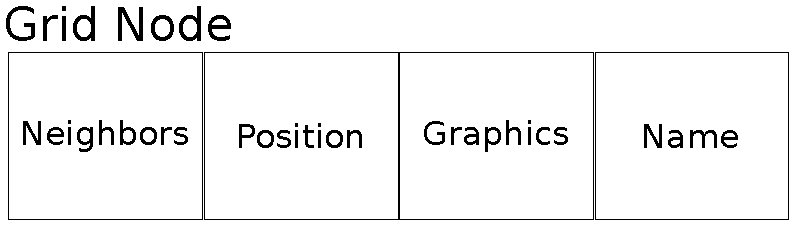
\includegraphics[width=10cm]{../img/grid-node.pdf}
    \caption{Memory representation of a grid node.}
    \label{grid-node}
\end{figure}

During the execution of the pathfinding algorithm, grid nodes get stored in cache for fast repeated access. The processor cache has a
concept of \emph{spatial locality}, which means that when it loads data from memory it loads a whole block of memory as spatially close
data are very likely to be accessed, too. However, a pathfinding algorithm only requires the list of neighbours of a node.
Figure~\ref{cache-inheritance} shows a possible cache state with four different grid nodes loaded. As we can see, quite a lot of unneeded
data was loaded to the cache due to spatial locality which can cause quite frequent cache misses because of the limited size of the cache.

\begin{figure}[H]
    \centering
    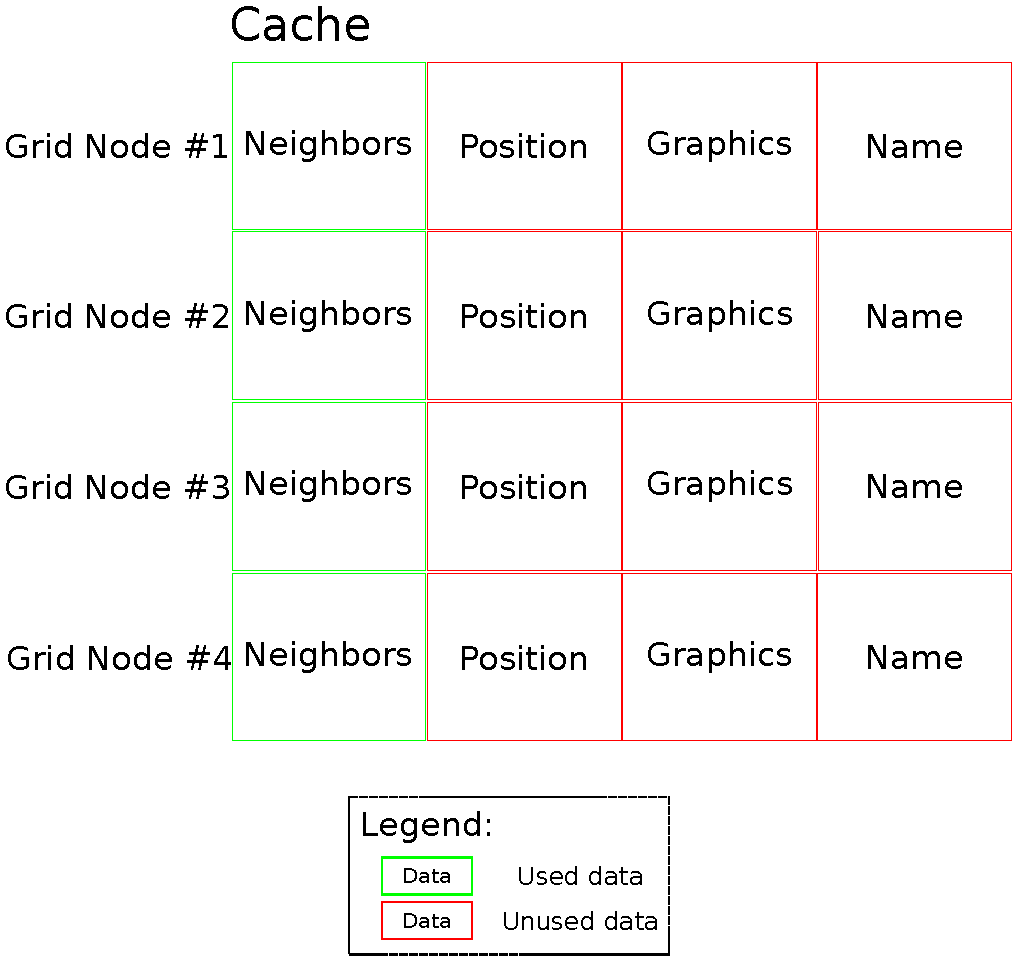
\includegraphics[width=9cm]{../img/grid-cache-inheritance.pdf}
    \caption{Example of a possible cache state during a pathfinding algorithm if we have data grouped by entity in memory.}
    \label{cache-inheritance}
\end{figure}

If, on the other hand, we would have data grouped in memory by their purpose as opposed to having them grouped by entities, the spatial
locality of cache could be used to prefetch data that will likely be used during the pathfinding algorithm. In Figure~\ref{cache-dd},
we can see the state of the cache at the same point of the algorithm, but with data being grouped by their purpose in memory
-- instead of having the different nodes with their data next to each other, we have all neighbor lists next to each other and
similarly for all other data that belong to grid nodes.

With this data grouping, any data loaded to cache during the algorithm is very likely to be relevant to future computation and as
such might lead to fewer cache misses.

\begin{figure}[H]
    \centering
    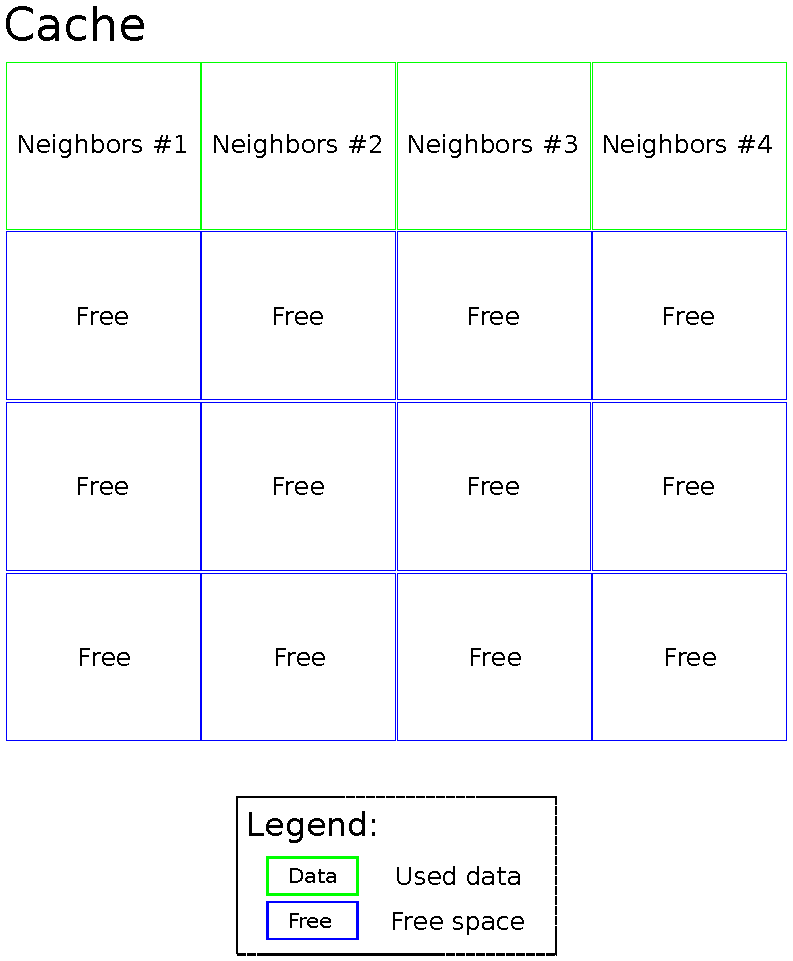
\includegraphics[width=9cm]{../img/grid-cache-data-driven.pdf}
    \caption{Example of a possible cache state during a pathfinding algorithm if we have data grouped by their purpose in memory.}
    \label{cache-dd}
\end{figure}

While it would be possible to incorporate such data grouping to this entity representation -- and it can lead to even 35\% increase
in performance in some cases~\cite{OOPPitfalls} -- the inheritance based entity representation suffers one additional performance
hit in the fact that, in \cpp, the use of a virtual function is slower than the use of a non-virtual one by about 25\%~\cite{CppProgLang} and
offers smaller opportunities for inlining.

Because of this, we think that if we were to use the spatial locality of cache, it might be better to use a representation that takes
it into account by itself.

\subsection{Entity Component System}

Entity Component System\footnote{Sometimes also referred to as Component Entity System.}~\cite{ECS-Wiki}~\cite{ScottBilasGDC}
~\cite{ECS-Gamedev}
-- often abbreviated as \emph{ECS} -- is a structural design pattern that endulges the \emph{composition over inheritance} principle.
It comprises three main elements: \emph{Entity}, \emph{Component} and \emph{System}.

\begin{itemize}
    \item Entity is an identifier of anything that is present in the game world. It can be as simple as a numeric 
        identifier or a more complex object, such as a component container.
    \item Component is a piece of logically related data, it generally represents a single characteristic 
        of an entity, such as its health, position, collision box, movement or behavior.
    \item System updates a single component or a set of components of all entities that have these components.
\end{itemize}

\begin{listing}[h]
    \centering
    \begin{lstlisting}
entity = {
    health_component = {
        health = 50,
        max    = 100,
        regen  = 2
    }
}

health_system = {
    components = { entity.health_component },

    function update()
        for comp in components do
            if comp.health < comp.max then
                regenerate(comp)
            end
        end
    end,

    function regenerate(comp)
        regenerated = comp.health + comp.regen
        comp.health = min(comp.max, regenerated)
    end
}
    \end{lstlisting}
    \caption{A simple health system that regenerates the health of every entity
            that has a health component.}
    \label{ecs-example}
\end{listing}

In Listing~\ref{ecs-example}, we can see an example of a system that -- on a set period -- regenerates the health of all entities
that have a health component. The \emph{health\_system} iterates over all \emph{health\_components}, which contains all
data related to health and regeneration. Updating the game state in ECS is then done by updating all systems.

This representation satisfies all of our four requirements. Since entities are nothing but a set of components, we can specify
which types of components constitute an entity in a simple script and we can even create completely new types of entities
during runtime by creating a new identifier and assigning components to it.

Similarly, we can add new components and remove existing components of an entity, which allows modification of already existing
entities. As an example, we can add a movement component to a stationary entity to make it able to move. This, like the definition
of new entities, can be easily done at runtime.

In both of these cases -- modifying an existing or creating a new entity -- ECS provides more flexibility than the inheritance
based approach, because \cpp does not allow us to change the inheritance hierarchy without recompiling the engine, while
ECS allows any possible combination of components.

If we use numeric identifiers to represent an entity, we can easily interface our entities to Lua as all \cpp functions
called from Lua can take the identifier as their argument and then find necessary components in the component database.
This approach would avoid the necessity to implement object representation in Lua -- which does not support object oriented
programming by default.

An interesting characteristic of the ECS is its satisfiability of our last goal -- performance. To store our components,
we often use some kind of a key value associative container, where the key is the entity identifier and the value is the component.
If our entity is not a numeric identifier, but a component container, it then contains pointers or references to the components
stored in this cenral container. Since logically related data -- components of the same type -- are located next to each other
in memory, we can then use spatial locality of cache to avoid some of the possible cache misses when we operate on components of a specific
type, because the blocks of memory loaded to cache are less likely to contain data that are irrelevant to the current computation.

\subsection{Conclusion}

The ECS representation, unlike the inheritance based one,  satisfies all of our requirements. It also offers greater modifiability and
allows easy entity interfacing to Lua scripts and because of these traits was chosen for our engine.

\section{Libraries}

In this section, we are going to examine different libraries that can be used in our game
to help us with its development.

\subsection{3D Rendering}

Since, according to our main goal, we are going to create a 3D game, the first library we need to choose is a 3D rendering library.
Our game will, similarly to the original Dungeon Keeper, only have a relatively small amount of visible entities in the game world: 
minions, enemies, spells, buildings and walls. Because of this, we will settle with a relatively small functionality of the library.
It will have to be able to load models created in a graphical editor so that our players can easily create new models and load them
in their mods  of our entities, render them to the game window and move them in the game world. In particular, the library should be
compatible with models created in Blender~\cite{Blender}, which is fairly popular, has a lot of documentation and is free, which means
there will not be an additional cost of purchasing a graphics editor license to create models for our game.

Additionally, since our design element \textbf{(E4)} is the combat between our minions and enemies, support for animation
\footnote{Even though animation was planned for the game, it was not implemented because of time constraints.} would be
beneficial so that the combat is visible. Another of our design elements, \textbf{(E5)}, is the participation of the player in combat
by the use of spells. This feature will require the ability to transform rendered objects to create spell effects such as explosions.

Another important aspect of a library is the ease of its use. Because of this, our chosen library should provide an easy to use
interface, have complete and clear documentation and a large enough community.

Lastly, the library should be compatible with our ECS entity representation because the model of an entity is part of its data and
as such will need to be part of one -- or some -- of its components.

\subsubsection{Low level API: OpenGL and DirectX}

Lower level API provides direct acces to the graphics hardware, common examples are OpenGL and DirectX. These interfaces, while
extremely flexible, do not support models created in an external application and thus fail to satisfy one of our goals. Additionally,
if we decided to use one of these interfaces, we would need to implement a lot of functionality -- such as scene representation -- that 
is already provided to us by a higher level library and thus would prolong the development time of our game. For these reasons, we would
like to find a library that provides these features.

\subsubsection{Higher level API: Ogre3D and Irrlicht}

Another option is a higher level API, which is often a wrapper around
a lower level API such as OpenGL and DirectX. The benefit of this option is that a higher level API often provides a large amount
of already implemented functionality and data structures which a lower level API does not. For this decision, we retain all of our
requirements for the choice of our rendering
library and add an additional one -- the higher level API should be able to wrap aroung both OpenGL and DirectX. The reason for this is
that a common problem a user encounters when using a 3D application is related to drivers. Allowing the user to switch the underlying
API used in case of program crashes might solve these problems~\cite{BothOpenGLAndDirectX}.

We took two libraries into consideration -- Ogre3D~\cite{Ogre3D} and Irrlicht~\cite{Irrlicht}. These were selected because they both have
been previously used to create commercially successful games -- Torchlight~\cite{Torchlight} and Octodad~\cite{Octodad}: Deadliest Catch, 
respectively.
Both of the considered libraries satisfy all of our requirements as they both
support models created in an external application and their manipulation at runtime, provide complete and clear API documentations,
both have large communities, wrap around both OpenGL and DirectX and provide an object representing a loaded model which can be
integrated into a component in our ECS entity representation and can be easily interfaced to Lua. One difference between Ogre3D and Irrlicht
is that an application that uses Ogre3D provides its user with a configuration window on startup, where the user can choose -- along with
other graphics options -- which underlying API they would like to use. If we use Irrlicht, we would need to implement this configuration
window ourselves.

Another difference between these two libraries is in the way they are integrated into our application. If we choose Irrlicht, we would need
to create the game's main loop and call Irrlicht to draw our models. If, on the other hand, we use Ogre3D, the main loop is handled by Ogre3D
and we only provide callbacks that update the game and handle events. While this difference might not seem significant, we think that
the event handling done through different callbacks makes it easier to implement input handling and results into easier to read source
code, since we do not need to check the type of an event and instead provide different handlers for different events -- e.g.
a key press, key release, mouse movement or mouse click.

These, albeit small, two differences were the reasons for choosing Ogre3D, since we think that these two libraries are equal
on a technical level and the use of both would reach similar results.

\subsection{Graphical User Interface}

Now that we have chosen our 3D rendering library, we need to choose a library that provides tools to create a Graphical User Interface 
-- often abbreviated as \emph{GUI}. The main requirement for the library is its compatibility with Ogre3D as they will both need to render
to the same window. Since this library will be used to create the interface our players will use to control the game,
it has to offer widgets that will allow for control of all our design elements including, but not limited to:

\begin{itemize}
    \item Button -- needed for spell and building choosing and research.
    \item Label -- needed to display current amounts of the game's resources.
    \item Frame -- needed as a background for other widgets.
\end{itemize}

Aside of these three, the library should also contain widgets that would allow us to create in game console -- that is an edit box, 
text box and a scroll bar -- which would be beneficial for testing and prototyping. Lastly, to allow modifications of our GUI, an external 
GUI editor that can be used to create configuration files representing the GUI of our game would be beneficial.

\subsubsection{Ogre Overlay}

Overlays are a feature of the Ogre3D library which allows us to render 2D and 3D elements on top of the normal scene. It can be used to
create windows, buttons, labels and other widgets but does not provide already prebuilt widgets. This would mean that we would need
to implement all the widgets we need along with a system that handles the interaction between the user and our GUI.

While this option does not require any additional library to be used in our project, the development cost would be too high
when compared to a GUI library that already provides these widgets as well as means for input handling. Because of this and the lack of
an external GUI editor, we decided to use a dedicated GUI library in our game.

\subsubsection{CEGUI}

CEGUI~\cite{CEGUI} is a GUI library that was originally a part of the Ogre3D library and as such is fully compatible with it. The library
provides a wide array of different widgets, including all of the one we require and many more.

To create our GUI schemas, we can use the Unified Editor for CEGUI~\cite{CEED}, which generates XML files that contain information
about our scheme such as the position, size or text of our widgets. Our mod creators can modify these XML files to modify our GUI.

Because CEGUI satisfies all of our goals and because it was previously bundled with Ogre3D -- meaning there are tutorials, documentation
and community discussions related to the integration of these two libraries -- we decided to choose CEGUI as the GUI library for our game.

\section{Pathfinding}

An important aspect of most games is the ability of entities to find the way to their target inside the game world. This is done through
a process called \emph{pathfinding}. From a programming point of view, pathfinding is a process of finding -- often the cheapest -- path
inside a pathfinding graph. Since our game, similarly to the original Dungeon Keeper, is tile based -- meaning that the game world
is divided into a set of adjacent square tiles, each representing a node in the pathfinding graph -- our pathfinding graph will have the
form of a grid. Nodes in this grid will be connected by edges to all of their neighbours. Nodes can be in the corner, on the side
or inside the pathfinding graph and have three, five or eight neighbours, respectively.

We now need to decide which algorithm we are going to use for pathfinding. Since diagonal edges between nodes are visually longer than
non-diagonal ones, the algorithm needs to work on a pathfinding graph with weighted edges. Additionally, pathfinding will be performed
quite often and as such our algorithm must try to avoid searching the entire pathfinding graph to find a suitable path.

The algorithms we took into account are the Dijkstra's algorithm, the breadth-first search and depth-first search algorithms 
-- often abbreviated as \emph{BFS} and \emph{DFS}, respectively -- and the A* algorithm. Out of these options, we decided to choose
the A* algorithm as it works on weighted graph and uses a heuristic to avoid unnecessary searching. The BFS and DFS algorithms failed
to satisfy our requirement that the algorithm should work on weighted graph and the Dijkstra's algorithm, while working on weighted
graphs, does not use a heuristic to avoid examining some of the nodes and tends to run slower than A*.

\section{Levels and serialization}

To satisfy our goal \textbf{(G2.3)}, our game has to provide the ability to create custom levels that can be distributed by
players and then loaded by other players. Unlike the original Dungeon Keeper, which had a predefined set of levels, our game uses
randomly generated levels. The primary reason why we chose this change is that we believe that randomly generated levels can extend the
replayability of our game -- since the amount of different levels is not limited to a small set. The secondary reason is the nature of
our game -- the player is the one that shapes the world by building their dungeon.

The impact of this decision is that we do not need to store our levels as they get created whenever the player starts a new game. 
Because of this choice, we are going to satisfy our goal \textbf{(G2.3)} through the means of serialization. By serialization, we mean
saving of the game's current state to a persistent file on the hard disk which can later be loaded back into the game and the player
can continue from the serialized point.

This way, if a player wants to create a custom map, they can generate a new level, modify it, serialize it and distribute the created
file to other players that can easily load it. Since we want to allow our users to create custom levels similar to the Team Fortress~2
map created in Minecraft that was presented in the introduction of this thesis, our only requirements -- besides saving the game's state --
is the ability easily edit these serialized files and through these edits change the state and mechanics of the game.

\subsection{Binary}

During a binary serialization, the game state -- in our case the components of entities and some additional information -- gets
serialized as a sequence of bytes into a binary file. While this option results in generally smaller save files than a text serialization,
it prohibits modification of the game's mechanics. Additionally, even though this format allows our players to modify the
serialized game state, these modification would require an application that would parse the save file, allow the user
to change the data and then serialize the data again.

\subsection{XML}

Another considered option, the Extensible Markup Language -- often abbreviated as \emph{XML} -- would allow us to serialize the
state of our game to a human readable yet easily parseable format. This would allow our players to easily change characteristics of the
serialized entities -- e.g. their health, position or types of components -- and even to add new entities or delete existing entities
from the game state.

However, similarly to the binary format, XML files cannot contain custom code that would alter the mechanics of our game.

\subsection{Lua}

The last considered option is serialization into Lua scripts, which means that our game generates a sequence of calls to our Lua
API that transforms an empty level to the serialized one and stores these calls into a source file that is then executed by Lua when
the player wants to load the level.

This option allows our players to use the entire modding API inside these save files, which means that
entire mods can be distributed in the form of a serialized game state which would satisfy our goal \textbf{(G3)}.
Additionally, this feature is very easy to implement because of our
entity representation. The game's state comprises the states of individual entities along with some additional information -- e.g.
state of the wave system, research and resources. This means that we only need to implement serialization of the different
components in the game along with the aforementioned additional information using the Lua API. Deserialization does not need to be explicitly
implemented as it constists of deleting the current game's state -- if any -- and executing a Lua script that represents the desired
game state.

This option has one major downside when compared to the other considered options -- the size of the scripts. With a very large world,
the serialized state of the game becomes too big and can cause long loading times and thus limits the size of the game world.
However, we do not consider this limitation too bad as we found smaller levels sufficient for general play.

\subsection{Conclusion}

While the first two options -- binary and XML serialization -- would allow us to serialize bigger worlds than we can with Lua scripts,
the ability to edit both characteristics of the serialized entities and the mechanics of the game that Lua serialization provides us
is, we think, worth the bigger size of the saved file when a large level gets serialized. Because of this, we decided to choose Lua script
generation as our serialization system.

\chapter{Implementation / Dev Docs?}
% TODO

\section{Engine (?Layout)}

% TODO
\begin{itemize}
    \item describe Component - System - Helper - LuaInterface - ... relationship
    \item possibly create a picture
    \item describe the "workflow" of the game? or leave it to other sections?
\end{itemize}

\section{Game}

% TODO
\begin{itemize}
    \item !ask PJ: do I have to describe functions even if they have documenting comments? 
    \item describe how the game is initialized
    \item explain OIS and Ogre callbacks (+ parent classes)
    \item brief description of its members vs just mentioning them vs ignoring them as they will be explained later?
    \item level creation (new\_level \&\& generate\_empty\_level)
    \item throne monitoring? (keeping throne ID so there is only one target of the enemies)
    \item possibly add a subsections describing Ogre and CEGUI initialisation
\end{itemize}

\subsection{State Design Pattern}

% TODO
\begin{itemize}
    \item describe the pattern
    \item describe the states of the game
    \item explain why the pattern is NOT used
\end{itemize}

\section{Components}

% TODO
\begin{itemize}
    \item go through components one by one with UML-like pictures describing theis members and purpose
    \item explain why strings are moved?
    \item explain why components need default values for every parameter of their constructor?
    \item go through some more complex concepts of the components (align states, maybe forward reference blueprints, etc.)
\end{itemize}

\section{Systems}

% TODO
\begin{itemize}
    \item define systems
    \item mention common base class and the reason for inheritance (list of systems...)
    \item describe the component-system relationship (none, system-component, system-components, systems-component, ...)
\end{itemize}

\subsection{CombatSystem}

% TODO
\begin{itemize}
    \item describe the update logic
    \item describe entity querying
    \item describe effect application
    \item talk about the fabulousness of the query \& effect design!
    \item talk about the run away mechanism?
    \item talk about runtime projectile creation?
    \item talk about line of sight and LoS wrt BB?
\end{itemize}

\subsection{EntitySystem}

% TODO
\begin{itemize}
    \item describe the update logic
    \item describe cleanup (and its delay and why it's necessary)
    \item id system (back then vs now)
    \item entity creation process
    \item component containers
    \item describe component manipulation (add, load, set, delete, delete now, ...)
    \item mention entity registration for the entity creator window
    \item describe function array (reason, jmp table bonus, etc.)
    \item explain the macros!
    \item describe why constructors are delayed (so that the lua function where it's create continues before constructor call)
    \item maybe talk more about component loading from lua? or leave that to the scripting part? or never mention it?
\end{itemize}

\subsection{EventSystem}

% TODO
\begin{itemize}
    \item describe the update logic
    \item describe event persistence/destruction
    \item describe how to make event one (successful) pass only
    \item targeted/area events and area event expansion
    \item delete component vs delete entity discussion
    \item describe handling (fixed C++ vs Lua)
    \item this should be first time we encounter update periods and time multipliers, explain!
\end{itemize}

\subsection{GridSystem}

% TODO
\begin{itemize}
    \item describe the update logic (+freed/unfreed and Grid relation)
    \item talk about grid graphics used for debugging?
    \item explain structure placement
    \item describe alignment checks
\end{itemize}

\subsection{TaskSystem}

% TODO
\begin{itemize}
    \item describe the update logic
    \item talk about busy state, processing tasks and checking if task is complete
    \item probably only forward reference the Lua part? or talk about it right here? !ask PJ!
\end{itemize}

\subsection{WaveSystem}

% TODO
\begin{itemize}
    \item describe states and maybe mention why the State design patter wasn't used (too simple)
    \item describe the update logic of the different states (-> countdown, spawning, chilling)
    \item talk about the spawning mechanism, blueprint vector, spawn nodes
    \item talk about wave entity monitoring and wave ending
    \item talk about the wave table
    \item talk about the wstart and wend callbacks
    \item talk about endless mode
    \item possibly explain how to write a wave? or add that to the scripting part?
\end{itemize}

\subsection{Other}

% TODO
\begin{itemize}
    \item here explain in alphabetical order the remaining systems
    \item say why these are not as important (that is, not important to be described) as the others
\end{itemize}

\subsubsection{AISystem}

% TODO
\begin{itemize}
    \item describe the update logic
    \item mention update forcing (in relation to the update period mentioned earlier)
\end{itemize}

\subsubsection{GraphicsSystem}

% TODO
\begin{itemize}
    \item say how it's supposed to maintain all manual graphics logic but atm only does explosions
        (since it's the only manual graphics object)
    \item describe the update logic
\end{itemize}

\subsubsection{HealthSystem}

% TODO
\begin{itemize}
    \item describe the update logic
    \item mention configurable regeneration period
\end{itemize}

\subsubsection{InputSystem}

% TODO
\begin{itemize}
    \item describe the update logic
    \item explain initial purpose and why it's not used atm
\end{itemize}

\subsubsection{ManaSpellSystem}

% TODO
\begin{itemize}
    \item describe the update logic (both mana regen and entity spell casting)
    \item possibly talk about the relationship between player spells and entity spells
\end{itemize}

\subsubsection{MovementSystem}

% TODO
\begin{itemize}
    \item describe the update logic
    \item talk aboud move and checked\_move (and can\_move\_to) and why checked is not used
        but can be from lua (and was intended for 1st person mode)
\end{itemize}

\subsubsection{ProductionSystem}

% TODO
\begin{itemize}
    \item describe the update logic
    \item explain how products are spawned and placed
\end{itemize}

\subsubsection{TimeSystem}

% TODO
\begin{itemize}
    \item describe the update logic (mention the multiple comps updated)
    \item explain time event handling (and use)
    \item explain time event advancements
\end{itemize}

\subsubsection{TriggerSystem}

% TODO
\begin{itemize}
    \item describe the update logic
    \item explain how triggering works and why it works that way (factions)
    \item explain the general trap concept?
\end{itemize}

\section{Helpers}

% TODO
\begin{itemize}
    \item describe what helpers are and how are they used
    \item forward reference the not-singleton status of EntitySystem?
    \item explain why they were created (use in Lua and optionally in C++
        for better code readability)
    \item explain why they are slower than direct component manipulation
    \item explain component-helper relationship
    \item mention the general structure of a helper
    \item maybe talk about why they are namespaces and not classes?
        (+ namespace -> allows static class without any change basically)
\end{itemize}

\section{Script}

% TODO
\begin{itemize}
    \item talk about how it works (it's basically a wrapper facade)
    \item mention lpp::Exception
    \item explain the Lua C API (only informative? add a new section with a tutorial?
        tell the reader to read the Lua Programming Language 3rd edition book?)
    \item maybe go through some of the more complex functions?
\end{itemize}

\section{LuaInterface}

% TODO
\begin{itemize}
    \item talk about why it's needed (Lua needs static)
    \item talk about why it's centralised in one class?
\end{itemize}

\subsection{Initialising the API}

% TODO
\begin{itemize}
    \item explain the C++ function binding process
    \item explain the Lua module hierarchy
    \item explain other aspects besides function binding
\end{itemize}

\subsection{Extending the API}

% TODO
\begin{itemize}
    \item explain the general body of the interface functions (stack, return etc.)
    \item (super) small tutorial on how to add new interface functions
\end{itemize}

\section{GUI}

% TODO
\begin{itemize}
    \item talk about the GUI hierarchy
    \item explain initialization
    \item explain CEGUI button binding? maybe in general CEGUI manipulation?
    \item explain save/load file listing
    \item mention the GUIWindow class, base class of the following GUI windows
    \item explain why it has escape\_pressed handler and does not use CEGUI handlers
        for that (would be needed for all subwindows, too much a hassle - also would
        probably disregard the conditional closing)
\end{itemize}

\subsection{Console}

% TODO
\begin{itemize}
    \item talk about how awesome it is during debugging
    \item explain how execution and printing works (+ the history concept?)
    \item explain why it does not execute lines but multi lines after the execute
        button is pressed
\end{itemize}

\subsection{EntityCreator}

% TODO
\begin{itemize}
    \item mention that currently it is used for entity placement and
        the creation part is supposed to be a graphical way to make entities that
        is not currently in the game
    \item explain how it works
    \item explain how it's used for testing
    \item maybe mention that this is where the registered\_entity from EntitySystem
        is used
\end{itemize}

\subsection{EntityTracker}

% TODO
\begin{itemize}
    \item explain how tracking works
    \item talk about why it's useful
    \item mention the upgrade, exp convert and delete functionality?
\end{itemize}

\subsection{ResearchWindow}

% TODO
\begin{itemize}
    \item explain initialisation, how it works
    \item explain dummy\_unlock and its relationship with serialization
\end{itemize}

\subsection{Other}

% TODO
\begin{itemize}
    \item say that these are generally not that complex and quite straight forward
\end{itemize}

\subsubsection{BuilderWindow}

% TODO
\begin{itemize}
    \item talk about building registration (how it relates to unlocking)
    \item talk about the assembly line (also used in spell casting window)
        and why it's good (lack of images -> buttons need to be big and readable)
    \item don't forget to mention that this is just a graphical front end
        to EntityPlacer (with price management etc.) as is EntityCreator (though
        that one ignores price, and has all unlocked even enemies)
\end{itemize}

\subsubsection{GameLog}

% TODO
\begin{itemize}
    \item just mention that it is basically the ingame chat posting info
        for the player
    \item also maybe again mention history (same as console)?
\end{itemize}

\subsubsection{MessageToPlayerWindow}

% TODO
\begin{itemize}
    \item talk about button renaming and action assignment
    \item then mention how to use this as a whole
\end{itemize}

\subsubsection{OptionsWindow}

% TODO
\begin{itemize}
    \item talk about actions, key bindings and video settings
        (+ how they are done?)
\end{itemize}

\subsubsection{SpellCastingWindow}

% TODO
\begin{itemize}
    \item talk about spell registration (how it relates to unlocking)
    \item just mention the assembly line (already explained in BuilderWindow)
    \item talk about the relationship with the SpellCaster and how spell casting
        works on this side (simple invoking of the spell caster and marking
        the spell as active if needed)
    \item don't forget to mention that this is just a graphical front end
        to SpellCaster basically
\end{itemize}

\subsubsection{TopBar}

% TODO
\begin{itemize}
    \item just say something about its purpose (monitoring of resources)
\end{itemize}

\section{SpellCaster}

% TODO
\begin{itemize}
    \item discuss the spell casting concept in the game
    \item mention the spell types
    \item explain why it's so damn cool (ease of spell creation, run time spell creation)
    \item forward reference the Lua spell structure, which is explained later in Scripting
\end{itemize}

\section{Utilities}

% TODO
\begin{itemize}
    \item just say that these are classes that are not directly part of
        the game world but are used as background tools that support the game
\end{itemize}

\subsection{Camera}

% TODO
\begin{itemize}
    \item talk about how it allows free/nonfree mode, resetting
        and backups
    \item maybe talk more about the free nonfree mode and how to toggle them
        (both keybind and command)
\end{itemize}

\subsection{Effects}

% TODO
\begin{itemize}
    \item talk about how awesome they are and allowed the creation of
        extensible effect application framework in CombatSystem
    \item explain how to write one
    \item mention that they are used as template arguments and as such
        should conform the given interface (also explain that)
    \item maybe ilustrate their structure on one of them
\end{itemize}

\subsection{EntityPlacer}

% TODO
\begin{itemize}
    \item explain its purpose and how it works
    \item explain why only the graphics component data is used (so it's ignored
        by the game world and serializer, etc.)
\end{itemize}

\subsection{LevelGenerator}

% TODO
\begin{itemize}
    \item explain their purpose and how to write one
    \item mention the cycle count constructor parameter
    \item mention the default tables in config (and that it's easy to add new ones)
\end{itemize}

\subsubsection{RandomLevelGenerator}

% TODO
\begin{itemize}
    \item say that this is just naive algorithm for a pseudo random level generation
        using number of neighbours that are gold deposits to determine if a gold
        deposit should be spawned
\end{itemize}

\subsection{RayCaster}

% TODO
\begin{itemize}
    \item explain that I'm a noob that stole other programmer's idea for this
        from the Ogre wiki
    \item explain why it's needed (polygon precision ray casting -> half cubes,
        without it only bounding boxes are checked and free space is impenetrable)
\end{itemize}

\subsection{SelectionBox}

% TODO
\begin{itemize}
    \item explain its purpose and how it works
    \item talk about single/area selection and multi selection using shift
\end{itemize}

\subsection{Conditions}

% TODO
\begin{itemize}
    \item explain their purpose, how they are used in querying and effect application
    \item mention that it's a good way for extensibility as new can be easily implemented
    \item mention that they are often used as template parameters and thus need to
        conform an interface (but not by inheritance)
    \item talk about the interface
    \item maybe demonstrate on an example
\end{itemize}

\section{Pathfinding}

% TODO
\begin{itemize}
    \item recapitulate form analysis that a modifiable function was used
        that allows different algorithms, heuristics and path types
    \item mentions its parameters (destruction, add path are primary!)
    \item mention how destruction works
    \item mentions why path addition is optional (for checks)
\end{itemize}

\subsection{Grid}

% TODO
\begin{itemize}
    \item explain its purpose and implementation
    \item mention that it only provides a set of grid related operations
        on a set of IDs it's provided (and assumes those are grid)
    \item mention random node placement and entity distribution
    \item mention free node list for ease (and speed) of access
    \item explain graph creation and linking
    \item explain general usage
\end{itemize}

\subsection{Algorithms}

% TODO
\begin{itemize}
    \item explain how they should be implemented (what functions, as they
        are used as template parameters)
    \item mention that A* is the only currently implemented
    \item mention portal implementation
    \item mention difference in complexity (component lookups)
    \item mention any other differences from a general A*
\end{itemize}

\subsection{Heuristics}

% TODO
\begin{itemize}
    \item explain how they are used and why they are inheriting a base class
        while other functors are not (state needed for some -> run away heuristic)
    \item maybe demonstrate on an example as the code is small?
\end{itemize}

\subsection{Path Types}

% TODO
\begin{itemize}
    \item explain what these things are and when they are used to check
        if the algorithm should stop
    \item explain their effect on the A* algorithm
\end{itemize}

\section{Serialization}

% TODO
\begin{itemize}
    \item talk about how easy component serialization is and how
        to create template specializations for new components
    \item show an example?
    \item explain the whole saving process, ents to be destroyed, unlocks,
        player, grid etc.
    \item explain the loading process
\end{itemize}

\section{Player}

% TODO
\begin{itemize}
    \item just say that it is used as a resource bank, keeping track
        of gold, mana, units etc
    \item mention that it also holds the starting unlocks used for new games
        (saved there during the game initialisation)
\end{itemize}

\section{Singleton Design Pattern}

% TODO
\begin{itemize}
    \item explain what this stuff is, its pros \& cons
    \item mention that the main reason for its use in this game
        is having one instance, not that much global access
\end{itemize}

\subsection{Script}

% TODO
\begin{itemize}
    \item mention how two Lua virtual machines cannot communicate
        and data are bound to C++ (via EntitySystem) so it's completely
        unnecessary to have more than one Scripting engine
\end{itemize}

\subsection{GUI}

% TODO
\begin{itemize}
    \item why would we want to have two GUIs?
    \item mention that here is the global access very good for testing?
\end{itemize}

\subsection{Player}

% TODO
\begin{itemize}
    \item why would we want two sets of player resources?
    \item serialization preserves them and shown is only the main set
        (also used is only the main one)
\end{itemize}

\subsection{Grid}

% TODO
\begin{itemize}
    \item explains how it only operates on a set of given IDs that are
        made during graph creation (+ mentions it would be easy to implement
        their switch) so there does not need to be more than one pathfinding grid
    \item also mention that due to the nature of the game levels, it would be nonsense
        to have two grids
\end{itemize}

\subsection{EntitySystem}

% TODO
\begin{itemize}
    \item explain how even though it's getting passed around a lot (mainly Helpers),
        there could be a reason to use more than one EntitySystem instance (like a backup
        for example) and thus the Singleton pattern might not be the best choice
    \item maybe compare it to the 4 previous classes
\end{itemize}

\section{Scripting}

% TODO
\begin{itemize}
    \item talk about the API, possibly mention some API reference text file
        that I should make as an attachement
\end{itemize}

\subsection{Initialisation}

% TODO
\begin{itemize}
    \item talk about the config.lua \& init.lua duo
    \item explain different options in config
    \item explain how scripts packs are added to init
    \item talk abut the core.lua file of each script pack
        and what it should do (probably with an example)
    \item explain how to add a new script directory
    \item explain how to override some behaviour
    \item explain the new level callback and for what it can be used
        (+ the return value meaning)
\end{itemize}

\subsection{Entity Representation}

% TODO
\begin{itemize}
    \item explain the structure of a script representing
        an entity (with a small example)
\end{itemize}

\subsection{Blueprints}

% TODO
\begin{itemize}
    \item explain what is a blueprint, how to make one and
        how to use it
    \item explain why it's a table and not just a function
        and why the functions in different blueprint should
        have different names
\end{itemize}

\subsection{Research}

% TODO
\begin{itemize}
    \item explain how to add new unblocks and modify existing ones
\end{itemize}

\subsection{Spells}

% TODO
\begin{itemize}
    \item explain the structure of a spell table and how to make new spell
    \item mention again the spell types and the difference they make
        in the spell table function implementations
    \item mention that spells can be made during run time for testing
        purposes
\end{itemize}

\subsection{Creating a Mod (? Modification)}

% TODO
\begin{itemize}
    \item provide a simple tutorial on how to make a new mod
    \item possibly the tower defense one?
\end{itemize}

\section{Extending the Game}

% TODO
\begin{itemize}
    \item small sequence of tasks that are needed for a new feature addition
        (that is component, system etc.)
    \item idea: show how a TargetedComponent would be implemented, allowing
        handlers for targeting/untargeting and how this could be used to create
        a chess mod
\end{itemize}

%\chapter{User's Documentation}

TODO: Check if game introduction should be here for the player.

\section{System Requirements}

% TODO
\begin{itemize}
	\item this might be a problem as CEGUI \& Lua have basically no
		requirements and Ogre3D only needs OpenGL (I believe v3 and above)
\end{itemize}

\section{Installation}

% TODO
\begin{itemize}
    \item just simply go over the installing process
    \item might be nice to create an installer using something like InnoSetup!
    \item maybe include a note on how to install a mod?
\end{itemize}

\section{About the Game}

% TODO
\begin{itemize}
	\item say what it is
	\item explain basic elements of the game (building, commanding units, gold,
		man, spells, research etc.)
\end{itemize}

\subsection{??? Goal of the Game / Goal}

% TODO
\begin{itemize}
    \item explain how waves work and how to win/lose the game
\end{itemize}

\section{Controls and Options}

% TODO
\begin{itemize}
    \item go over default options and how to rebing them
    \item go over window mode \& resolutions
    \item mentions what the APPLY button does wrt key bindings
\end{itemize}

\section{Research}

% TODO
\begin{itemize}
    \item explain the concept in depth
    \item ?go over individual research unlocks?
	    (maybe just enumerate each row and say if it's a building, spell, effect etc
	    and mention where are these explained)
    \item effects (double production, kill all, level up etc) might be explained here as they
	    wouldn't get covered in buildings or spells
\end{itemize}

\section{Spells}

% TODO
\begin{itemize}
    \item explain the concept in depth
    \item explain how to use the spell assembly line
    \item explain how to use different types of spells
    \item ?go over individual spells?
\end{itemize}

\section{Buildings}

% TODO
\begin{itemize}
    \item explain how to build (assembly line already explained in spells)
    \item go over what the buildings in the game do
\end{itemize}

\section{Units}

% TODO
\begin{itemize}
    \item simply go over the production process
    \item maybe explain the different types of units in the game
\end{itemize}

%\chapter{User's Documentation}

TODO: Check if game introduction should be here for the player.
Possibly add system requirements.

\section{Installation}

% TODO
\begin{itemize}
    \item just simply go over the installing process
    \item might be nice to create an installer using something like InnoSetup!
    \item maybe include a note on how to install a mod?
\end{itemize}

\section{About the Game}

% TODO
\begin{itemize}
	\item say what it is
	\item explain basic elements of the game (building, commanding units, gold,
		man, spells, research etc.)
\end{itemize}

\subsection{Goal of the Game}

% TODO
\begin{itemize}
    \item explain how waves work and how to win/lose the game
\end{itemize}

\section{Controls and Options}

% TODO
\begin{itemize}
    \item go over default options and how to rebing them
    \item go over window mode \& resolutions
    \item mentions what the APPLY button does wrt key bindings
\end{itemize}

\section{Research}

% TODO
\begin{itemize}
    \item explain the concept in depth
    \item ?go over individual research unlocks?
	    (maybe just enumerate each row and say if it's a building, spell, effect etc
	    and mention where are these explained)
    \item effects (double production, kill all, level up etc) might be explained here as they
	    wouldn't get covered in buildings or spells
\end{itemize}

\section{Spells}

% TODO
\begin{itemize}
    \item explain the concept in depth
    \item explain how to use the spell assembly line
    \item explain how to use different types of spells
    \item ?go over individual spells?
\end{itemize}

\section{Buildings}

% TODO
\begin{itemize}
    \item explain how to build (assembly line already explained in spells)
    \item go over what the buildings in the game do
\end{itemize}

\section{Units}

% TODO
\begin{itemize}
    \item simply go over the production process
    \item maybe explain the different types of units in the game
\end{itemize}


%\chapter*{Conclusion and Future Work}
\addcontentsline{toc}{chapter}{Conclusion and Future Work}


%%% Bibliography
%%% Bibliography (literature used as a source)
%%%
%%% We employ bibTeX to construct the bibliography. It processes
%%% citations in the text (e.g., the \cite{...} macro) and looks up
%%% relevant entries in the bibliography.bib file.
%%%
%%% The \bibliographystyle command selects, which style will be used
%%% for references from the text. The argument in curly brackets is
%%% the name of the corresponding style file (*.bst). Both styles
%%% mentioned in this template are included in LaTeX distributions.

\bibliographystyle{plainnat}    %% Author (year)
% \bibliographystyle{unsrt}     %% [number]

\renewcommand{\bibname}{Bibliography}

%%% Generate the bibliography. Beware that if you cited no works,
%%% the empty list will be omitted completely.

\bibliography{bibliography}

%%% If case you prefer to write the bibliography manually (without bibTeX),
%%% you can use the following. Please follow the ISO 690 standard and
%%% citation conventions of your field of research.

% \begin{thebibliography}{99}
%
% \bibitem{lamport94}
%   {\sc Lamport,} Leslie.
%   \emph{\LaTeX: A Document Preparation System}.
%   2nd edition.
%   Massachusetts: Addison Wesley, 1994.
%   ISBN 0-201-52983-1.
%
% \end{thebibliography}


%%% Attachments to the bachelor thesis, if any. Each attachment must be
%%% referred to at least once from the text of the thesis. Attachments
%%% are numbered.
%%%
%%% The printed version should preferably contain attachments, which can be
%%% read (additional tables and charts, supplementary text, examples of
%%% program output, etc.). The electronic version is more suited for attachments
%%% which will likely be used in an electronic form rather than read (program
%%% source code, data files, interactive charts, etc.). Electronic attachments
%%% should be uploaded to SIS and optionally also included in the thesis on a~CD/DVD.
\chapwithtoc{Attachments}

\openright
\end{document}
